% Preamble
\documentclass[11pt]{article}

% Packages
\usepackage{amsmath}
\usepackage{amssymb}
\usepackage{hyperref}
\usepackage{caption}
\usepackage{graphicx}
\usepackage{float}


\graphicspath{ {./images/} }

% Document
\begin{document}

    \tableofcontents


    \section{Introduccion}\label{sec:introduccion}
    El siguiente trabajo presenta el desarrollo de la implementacion, simulaciones realizadas y analisis de resultados de
    automatas celulares, en particular el juego de la vida y alteraciones del mismo.

    Con fines de producir diversas simulaciones con el objetivo de detectar comportamientos y patrones, se ha realizado
    simulaciones tanto en dos y tres dimensiones, modificando a su vez parametros de entrada.

    \section{Modelo}\label{sec:modelo}

    \subsection{Automatas celulares}\label{subsec:automatas-celulares}

    Un automata celular modela un sistema dinamico el cual evoluciona en pasos discretos mediantes reglas o heuristicas,
     las cuales determinan la transicion entre dos estados.

    El sistema se compone de una matriz de celdas que poseen un numero finito de estados discretos y estos se iran actualizando
    de manera sincronica en cada paso temporal.

    Las reglas se caracterizan por ser deterministicas y uniformes en tiempo y espacio. Es decir, que las reglas para la evolucion
    de una celda solamente depende de un vecindario. Donde este vecindario sera definido segun la implementacion y las reglas.

    En una transicion de estados, se define un alcance r, el cual determina el grupo de celdas cercanas que son tenidas
    en cuenta para la regla de transicion. Como es utilizado el valor r varia en funcion de la cantidad de dimensiones de
    la matriz y como se define el vecindario.

    \subsection{Definiciones de vecindad}\label{subsec:definiciones-de-vecindad}
    Como se ha mencionado, el alcance es un parametro que describe a un sistema en particualar. Sin embargo, debe tambien
    tenerse en cuenta bajo que definicion de vecindario se trabaja. Se han contemplado los siguietnes.

    En primer lugar el vecindario \textbf{Von Neumann} considera como vecina a aquellas celdas que se encuentran dentro del rango r
    considerando la distancia Manhattan. De forma mas precisa, el conjunto de vecinas se define de la siguiente manera
    $N_{i,j}^{vN}:=\{(k,l) \in L\ |\ |k-i|+ |l - j| \leq r\}$

    Por otro lado, el vecindario \textbf{Moore} considera una celda como vecina si toda las componentes de su posicion se encuentran
    a distancia menor a r. De forma mas precisa el conjunto de celdas vecinas es
    $N_{i,j}^{M}:=\{(k,l) \in L\ |\ |k-i|\leq r\ and\ |l - j| \leq r \}$.


    \subsection{Juego de la vida}
     Propuesto por John Horton Conway en 1970, el juego de la vida es un automata celular en dos dimensiones con las sigueintes reglas
    \begin{itemize}
        \item Se considera 8 vecinos (Vecindad de Moore, r = 1).
        \item Cada celda tiene dos estados posibles “Viva” o “Muerta” ($k=2$).
        \item Las Celdas Vivas, permanecerán vivas en el siguiente paso temporal si tiene 2 o 3 vecinos vivos, de lo contrario morirá.
        \item Las Celdas Muertas se transformarán en Vivas solamente si tiene exactamente 3 vecinos vivos.
    \end{itemize}

    \subsection{Juego de la vida}\label{subsec:juego-de-la-vida}



    \section{Implementacion}\label{sec:implementacion}


    \section{Simulaciones}\label{sec:simulaciones}

    \subsection{Parámetros de entrada}\label{subsec:parametros-de-entrada}

    Para poder llevar a cabo las simulaciones, se toma en cuenta un conjunto de parámetros de entrada.
    Los mismos se pueden categorizar entre fijos y variables, dependiendo de si su valor se mantiene
    constante a lo largo de todas las ejecuciones de la simulación para un mismo conjunto de reglas, o no.

    Comenzando con los parámetros fijos, se tiene los límites de la matriz ($border$),
    en el que se indican los valores máximos y mínimos de las coordenadas de las celdas en dos o tres dimensiones.
    Luego, se define la condición de vecindad a partir de dos parámetros:
    la forma en la que se consideran las celdas vecinas a una celda en particular, según los modelos mencionados
    en~\ref{subsec:definiciones-de-vecindad} ($condition$), y el alcance de la vecindad ($r$).
    Con respecto a las reglas de juego, se cuenta con dos parámetros que determinan las posibles cantidades de
    vecinos que debe tener una celda para que se mantenga viva ($shouldKeepAlive$),
    y para que una celda muerta se convierta en viva ($shouldRevive$); ambos son listas de enteros.
    Por último, se determinó el dominio inicial ($initialDomainProportion$), el
    cual representa una proporción del área, si es un simulación en dos dimensiones, o del volumen,
    si es en tres dimensiones, total de la matriz donde se generan las celdas vivas en el paso temporal 0.
    Es decir, siendo $A$ el área o volumen total de la matriz, el dominio inicial es $A \times initialDomainProportion$.

    Por otro lado, los parámetros que se varían a lo largo de las simulaciones son la cantidad de pasos temporales
    máximos ($maxIter$), y la proporción de densidad de celdas vivas en el dominio inicial ($initialLiveCellsProportion$),
    siendo este último un valor entre 0 y 1.


    \section{Resultados}\label{sec:resultados}
    A continuación, se presentan los casos de estudio que se han realizado para diferentes simulaciones del juego
    de la vida en dos y tres dimensiones, y sus respectivos resultados.
    Para cada caso, se detallan los parámetros de entrada fijos utilizados, seguido de una o más figuras en el que
    se muestra la evolución del sistema en cada paso temporal en valores extremos, y finalmente, un análisis del
    observable en función de la densidad de celdas vivas en el dominio inicial.

    \subsection{Conway en 2D}\label{subsec:conway-en-2d}

    Como primer modelo, se ha estudiado el reconocido juego de la vida de Conway en dos dimensiones.
    Para ello, se fija los siguientes parámetros de entrada:

    \begin{itemize}
        \item $border = (0, 0) \times (100, 100)$
        \item $condition = MOORE$
        \item $r = 1$
        \item $shouldKeepAlive = [2, 3]$
        \item $shouldRevive = [3]$
        \item $initialDomainProportion = 0.16$
    \end{itemize}
    Variando el parámetro $initialLiveCellsProportion$ entre 0.1 y 0.9, se ha analizado la cantidad de celdas vivas
    a lo largo de los pasos temporales.
    \begin{figure}[H]
        \centering
        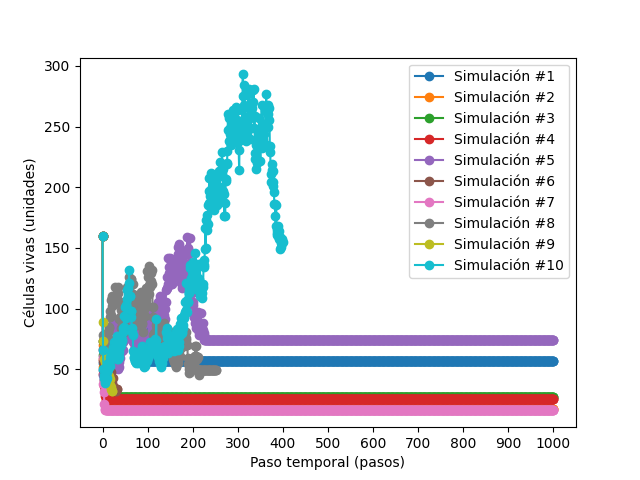
\includegraphics[width=0.6\linewidth]{conway2d/size_i10}
        \caption{Evolución en el tiempo del sistema de Conway con $initialLiveCellsProportion = 0.1$}
        \label{fig:conway2d_i10}
    \end{figure}
    \begin{figure}[H]
        \centering
        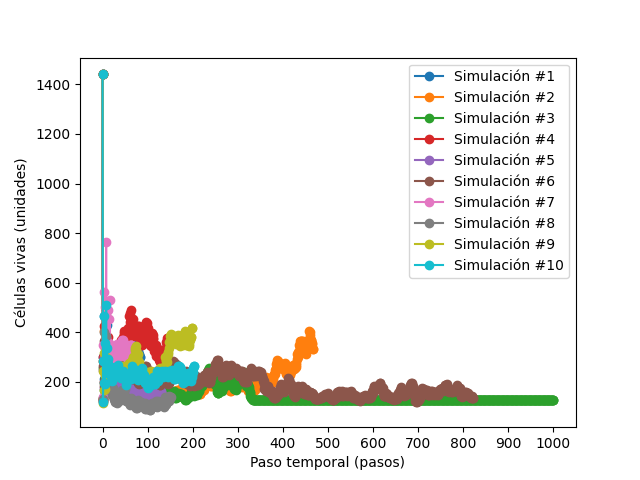
\includegraphics[width=0.6\linewidth]{conway2d/size_i90}
        \caption{Evolución en el tiempo del sistema de Conway con $initialLiveCellsProportion = 0.9$}
        \label{fig:conway2d_i90}
    \end{figure}

    \section{Conclusiones}\label{sec:conclusiones}


\end{document}